\chapter{\;\;\;\;Formal Semantics}
\label{sec:main-semantics}

%% ``\#'' 은 넣을지 말지 애매한 것들입니다.

%% \begin{enumerate}
%% \item Interaction semantics
  %% \begin{enumerate}
    %% \item genv 초기화
    %% \item state, step/call/return
    %% \item system call module (?)
  %% \end{enumerate}
%% \item C wrapper semantics
%%   \begin{enumerate}
%%   \item \cc{} 대충 설명
%%   \item typify (\ccc{}와 비교)
%%   \end{enumerate}
%% \youngju{typify will be explained later when we explain upper bound}
%% \item Asm semantics
%%   \begin{enumerate}
  %% \item \cc{} 대충 설명
  %% \item junk pointer와 callee-save checking
  %% \item memory permission (\ccc{}와 비교) \\
  %%    unfree temporarily breaks axiom but it is ok
  %% \item (\#) PC만 보고 call/step/return 구분하는 법 (\ccc{}와 비교)
%%   \end{enumerate}
%% \end{enumerate}

%% \todo{dummy stack?}

%% \youngju{\ccc{}는 메모리, state 분리해서 after external 같은게 메모리 안받는데 우리는 \cc{}와의 차이를 줄이기 위해 분리 안했다는 이야기 언급}



%% \begin{figure}
%%   \centering
%%   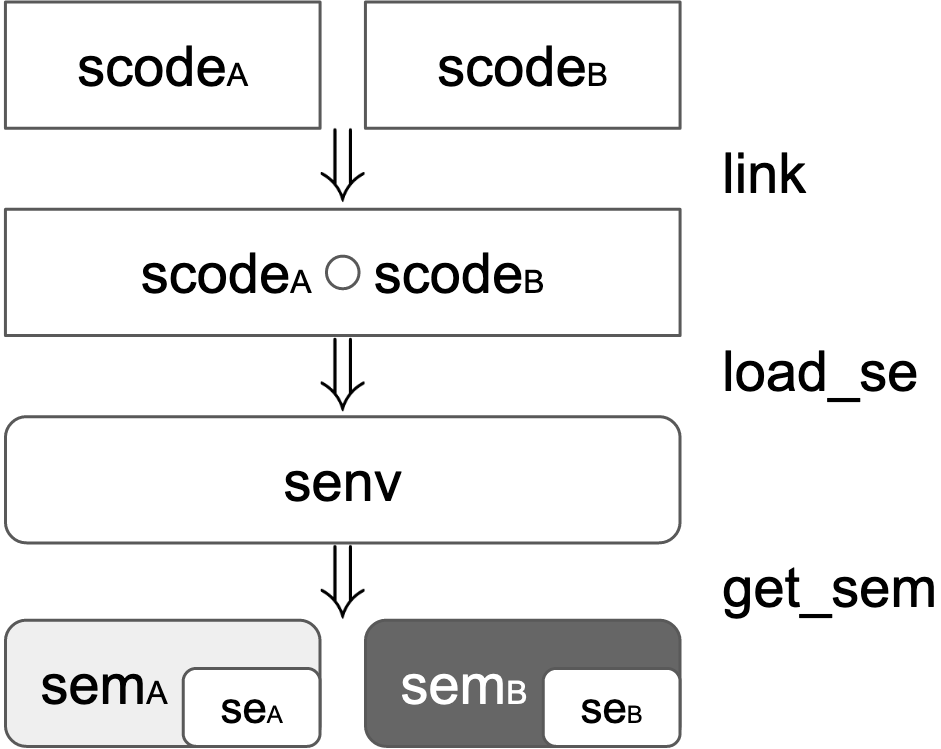
\includegraphics[width=0.25\linewidth]{fig-load.png}
%%   \caption{Loading Process}
%%   \label{fig:load}
%% \end{figure}



% Like \ccc{}, we require the set of states with \code{corestep}, states \code{at\_external}, and
% \code{halted} states are disjoint.  Second, unlike \ccc{}:



% Module semantics is almost same with \ccc{}. The differences are as follows.
% (i) While their primitives (\texttt{init\_core}, \texttt{at\_external}, \texttt{after\_external}, \texttt{halted}) were function, we use Prop instead.
% For \texttt{init\_core}, it is essential --- we have introduced nondeterminisim --- but for other cases, it is rather technical (and for uniformity with \texttt{init\_core}).
% Actually, we require the other three primitives are \emph{deterministic}, so it is equivalent with function.
% (ii) Our primitives change the memory, which is for marshalling/unmarshalling. In \ccc{}' marshalling/unmarshalling was hard-coded into \texttt{corestep} relation.
% (They already re-defined \texttt{corestep} for vertical compositionality.) In contrast, we just reuse off-the-shelf step relation from \cc{}.
% (iii) We support both C-style and Asm-style communications between modules, while \ccc{} only supported C-style.

% Currently, Asm-style communication is only allowed between Asm modules (this is the same for \ccx{}.

% Symbol code ($\Skel$) and symbol environment ($\Skenv$) represents \emph{language-agnostic} part
% of \cc{}'s program/global environment (as much as one can).
%% with one mild assumption --- each function has its signature --- which is true for all \cc{} languages.
% These are used in loading interaction semantics.  We use option signature type here.  The signature
% is none for the hand-written assemblies that does not follow (C-style?) calling convention, and for
% all other cases it is some.
%% We support both C-style and asm-style for call and return.

% We will skip explaining things that are same with \ccc{}.





% \myparagraph{Asm Wrapper Semantics}

% state recognition algorithm:
% \\ (1) PC points to my function --> corestep
% \\ (2) PC does not, but it is still in genv area --> call
% \\ (3) otherwise --> return

% Mention that unfree is somewhat special/nontrivial operation: it temporarily breaks \cc{}'s axiom, but it is okay.

% \begin{itemize}
%   \item init\_core:
%     \\ (1) c.(f) points to my function, fd. %% \cdashbox{It is declared as C-style and c is actually C-style} TODOOOOOOOOOOOOOOOOOOOO
%     \\ (2) PC <-| c.f
%     \\ (3) Allocate ``dummy'' stack with (size\_arguments fd.sig). Let its block id blk.
%     \\ (4) Fill in c.vs into blk
%     \\ (5) RSP <-| (blk, 0)
%     \\ (6) Assign junk blocks of arbitrary number
%     \\ (7) RA <-| arbitrary junk pointer outside genv area
%     \\ (8) Fill in other registers with junk pointer or arbitrary non-pointer
%   \item at\_external:
%     \\ (1) PC does not points to my function, but it is still in genv area.
%     \\ (2) From $se_{big}$, find signature of corresponding function.
%     \\ (3) Read list val from my arguments area, (vs).
%     \\ (4) Free my arguments area
%     \\ (5) c <-| (PC, current mem, vs)
%   \item after\_external:
%     \\ (1) $PC_{current}$ <-| $RA_{before}$
%     \\ (2) Make caller-save registers undef
%     \\ (3) RAX (return register) <-| r.v
%     \\ (4) Unfree my arguments area, and fill it with undef
%   \item final\_frame:
%     \\ (1) PC does not points to my function, and it is not in genv area
%     \\ (2) Check PC is same with initial RA
%     \\ (3) Do callee-save checking with inital registers.
%     \\ (4) Free my ``dummy stack''.
%     \\ (5) r <-| (r, current mem)
% \end{itemize}

% Mention we also support asm-style passing.
% As mentioned before, asm-style passing is only allowed between assembly modules.
% We just pass (both in call and return) current register set and memory directly.
% The only one exception is \textbf{RA} register: it exactly follows C-style convention, in order to use ``state recognition algorithm'' above.
% \textbf{RA} is \cc{}-specific pseudo register so we can do what we want.




%%% Local Variables:
%%% mode: latex
%%% TeX-master: "main"
%%% End:

